\normaltrue
\correctionfalse

%\UPSTIidClasse{12} % 11 sup, 12 spé
%\newcommand{\UPSTIidClasse}{12}

\exer{Broche de fraisage $\star$ \label{C2:10:Coh:528}}
\setcounter{question}{0}\UPSTIcompetence[2]{C2-10}
\index{Compétence C2-10}
\index{Torseur de cohésion}
\index{Diagramme des efforts intérieurs}

\ifcorrection
\else
\textbf{Pas de corrigé pour cet exercice.}
\fi

\ifprof
\else

La figure suivante verso illustre la cinématique permettant la rotation d'une broche de fraisage sur un centre d'usinage multiaxes.
On s'intéresse en particulier à l'arbre intermédiaire 2. Celui-ci est modélisé  par une poutre de diamètre $D$ et de longueur utile $L$. Les variations de diamètres seront négligées.

\begin{center}
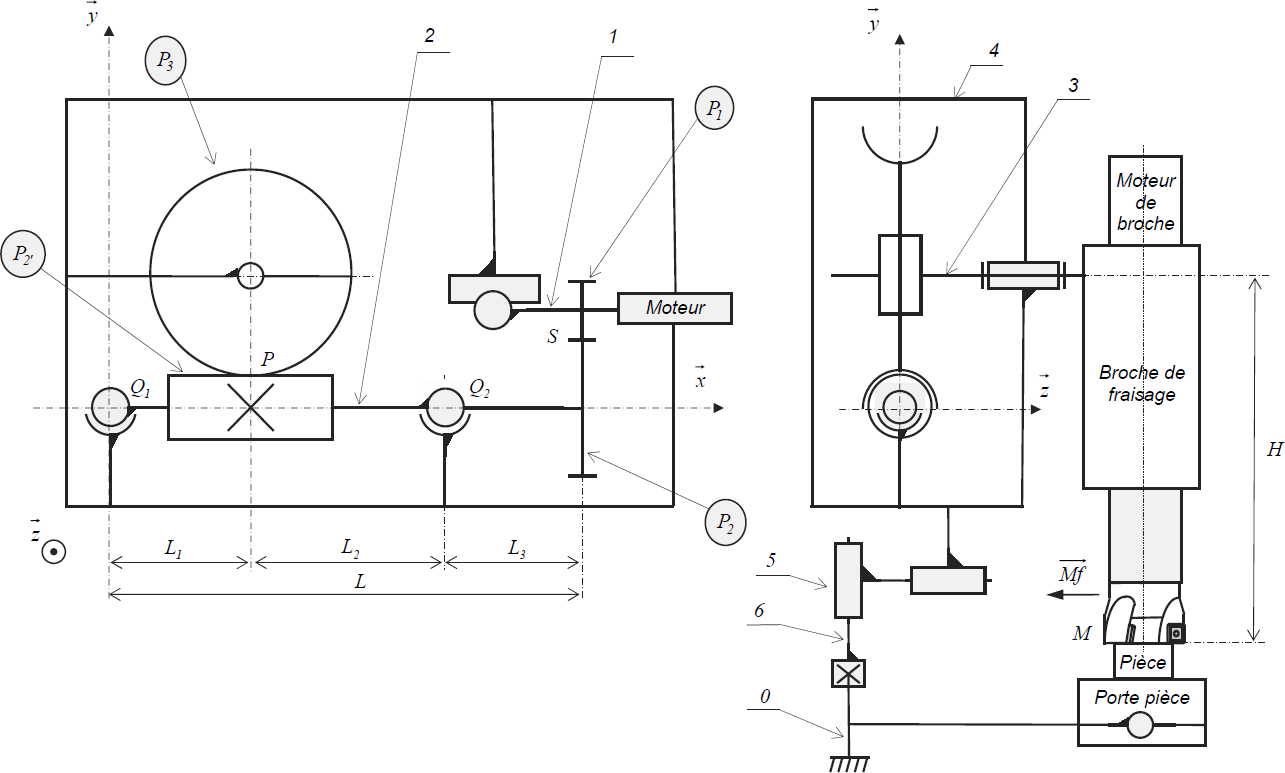
\includegraphics[width=\linewidth]{528_02}
\end{center}


\begin{center}
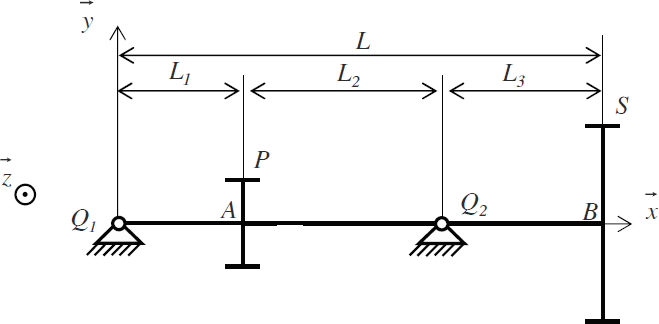
\includegraphics[width=\linewidth]{528_03}
\end{center}


Les points $A$ et $B$ sont les centres d’inertie géométriques des sections droites contenant
respectivement les points $P$ et $S$.
En considérant la composante $A_{32}$ des efforts de la roue sur la vis dans le sens $\vect{x}$ positif, les
torseurs des actions mécaniques extérieures qui s’exercent sur l’arbre intermédiaire 2, dans la base
$\base{x}{y}{z}$, sont :
$\torseurstat{T}{4}{2}_1 = \torseurcol{X_{Q_1}}{Y_{Q_1}}{Z_{Q_1}}{0}{0}{0}{Q_1}$, 
$\torseurstat{T}{4}{2}_2 = \torseurcol{X_{Q_2}}{Y_{Q_2}}{Z_{Q_2}}{0}{0}{0}{Q_2}$, 
$\torseurstat{T}{3}{2} = \torseurcol{A_{32}}{-R_{32}}{T_{32}}{0}{0}{0}{P}$, 
$\torseurstat{T}{1}{2} = \torseurcol{0}{-R_{12}}{-T_{12}}{0}{0}{0}{S}$.

\fi

\question{Proposer une méthode permettant de déterminer l'expression du torseur des efforts intérieurs au centre d'inertie de chaque section droite.}

\question{Mettre en \oe{}uvre cette méthode pour déterminer le torseur de cohésion.}

\question{Tracer les diagrammes des sollicitations en fonction de l'abscisse du centre d'inertie de la section droite.}

\subsection*{Torsion de l’arbre intermédiaire 2}

Le module de Coulomb du matériau utilisé est : $G = \SI{80000}{MPa}$.

\question{Déterminer l’expression, en fonction de $T_{12}$, $d_2$, $G$, $L_2$, $L_3$ et $\theta_{\text{lim}}$, du diamètre minimum $D_{\text{min}}$ de l’arbre 2, pour que le déphasage $\theta$ des sections passant par le point
$P$ et par le point $S$ soit inférieur à la valeur limite $\theta_{\text{lim}}$.}

\question{Dans le système étudié, le constructeur souhaite $\theta_{\text{lim}}=0,1\degres$. Donner la valeur
numérique de $D_{\text{min}}$.}

\question{Du fait de l’existence de ce déphasage de sections et vis-à-vis du système étudié, quelle
est le meilleur emplacement pour positionner le capteur de position. Doit-on le positionner
sur le moteur ou sur la broche elle-même ? Justifier brièvement votre réponse.}



\ifprof

\begin{center}
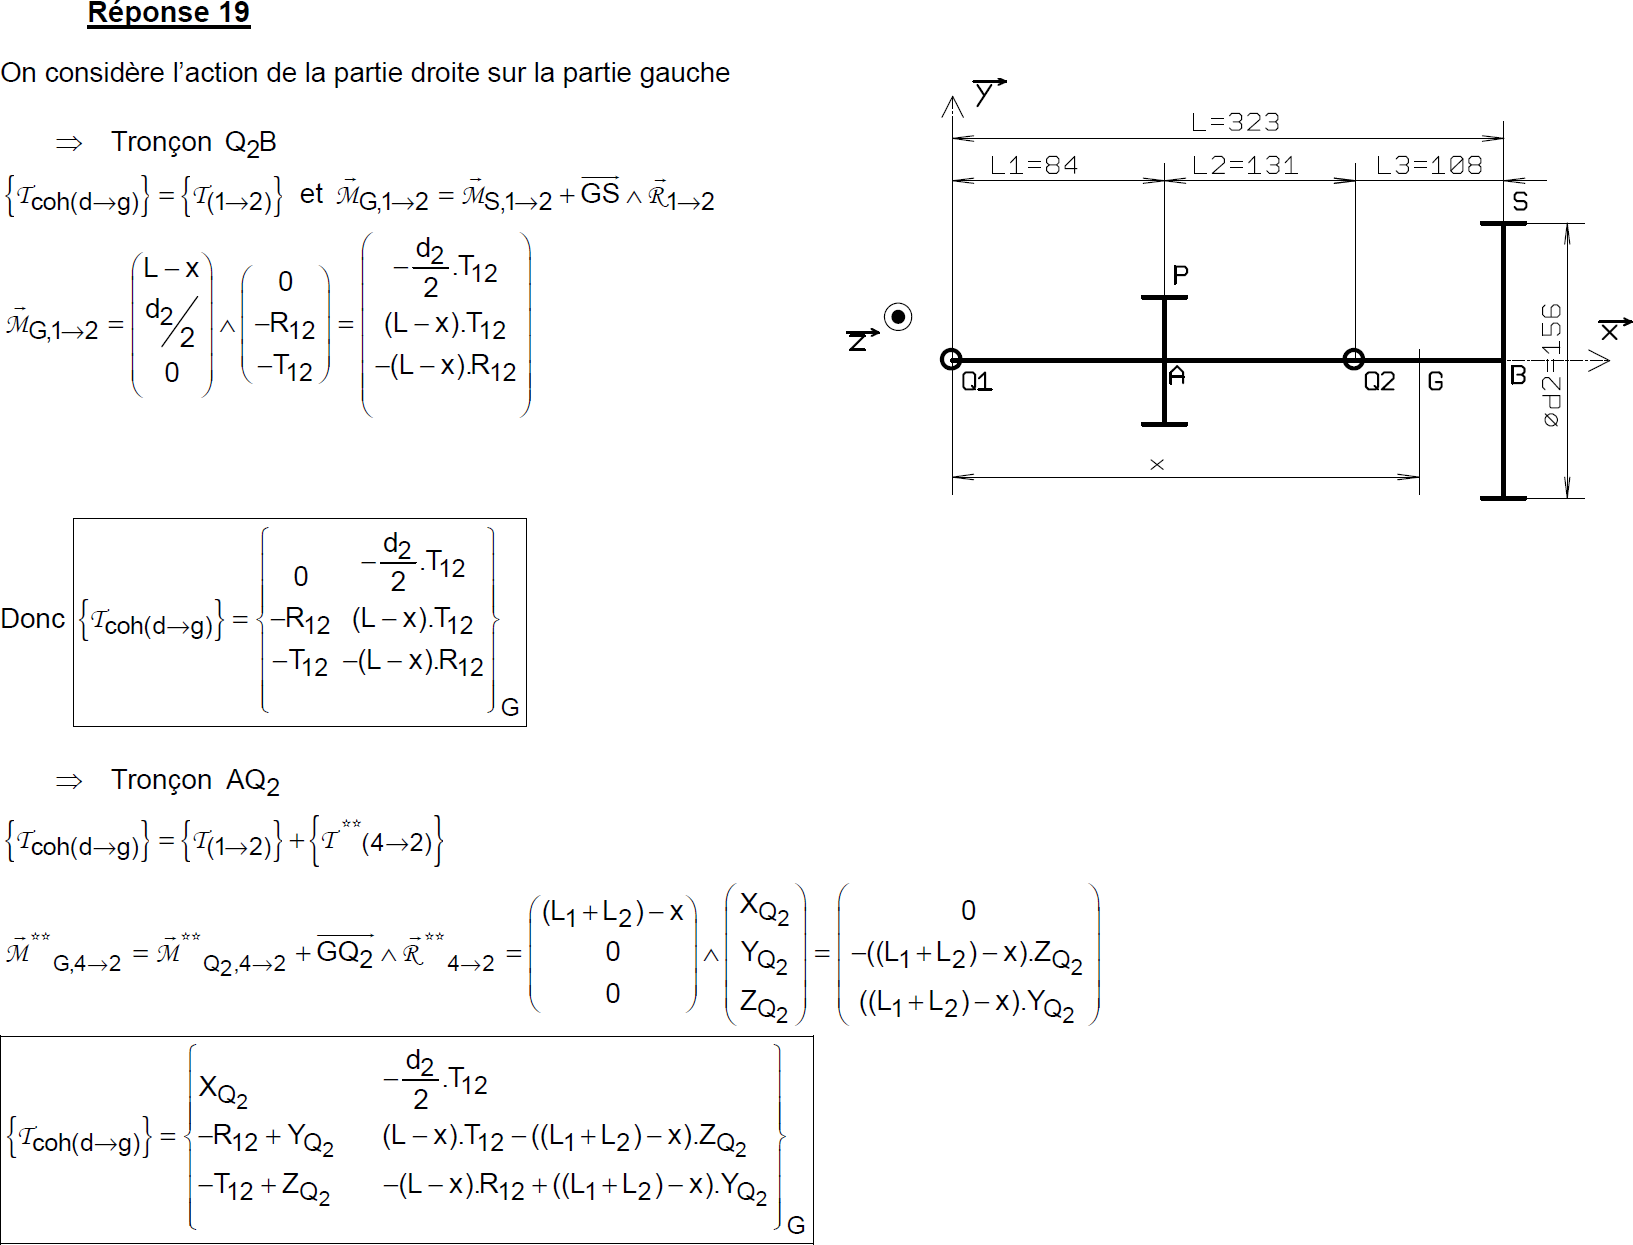
\includegraphics[width=\linewidth]{528_01_c}
\end{center}

\begin{center}
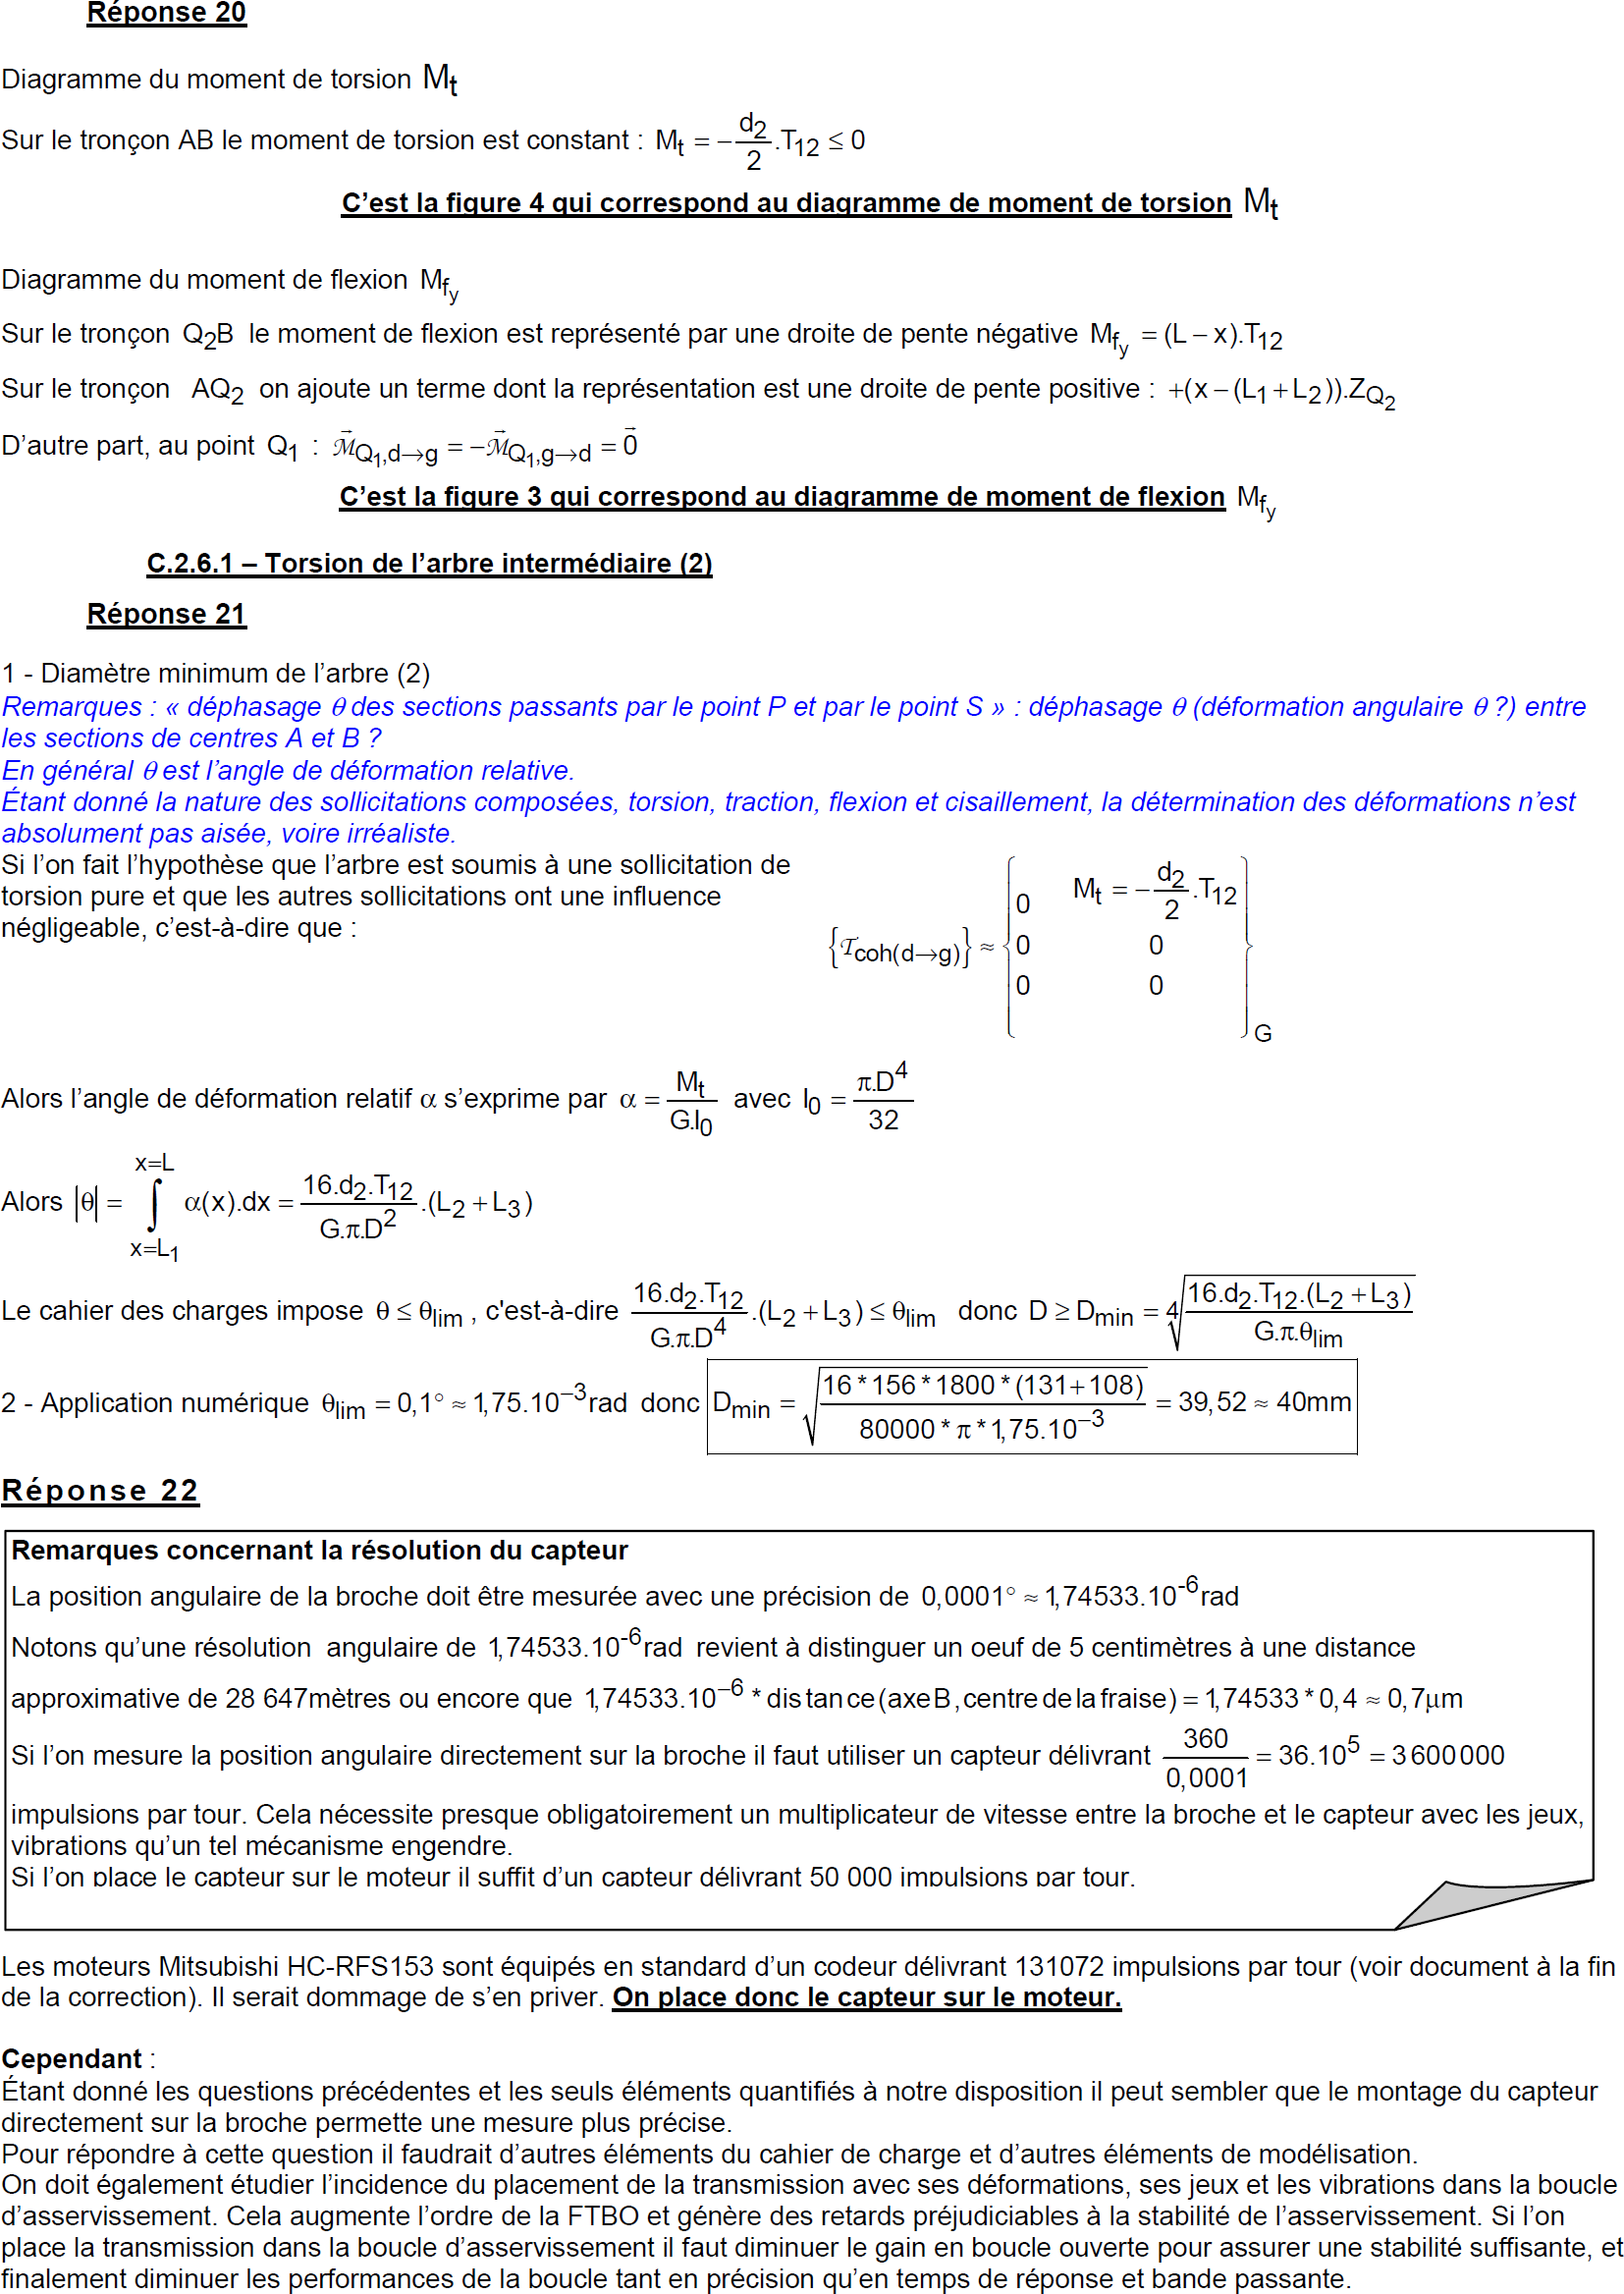
\includegraphics[width=\linewidth]{528_02_c}
\end{center}

\else
\fi


%\begin{figure}[H]
%\centering
%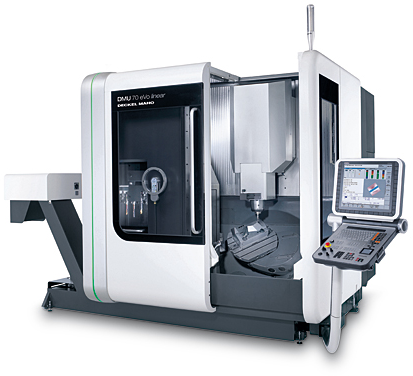
\includegraphics[width=\linewidth]{528_01}
%%\caption{\label{61_01} Loi de commande de vitesse en trapèze}
%\end{figure}


\ifprof
\else
\begin{flushright}
\footnotesize{Corrigé  voir \ref{C2:10:Coh:528}.}
\end{flushright}%
\fi

